% !TeX root = ../../main.tex
\section{Detailed calculations}
\label{app:reaction}

\subsection{Effectiveness factor}

The effective diffusional coefficient $D_e$ is first calculated to be 4.42 \times 10\textsuperscript{-10} using the widely-used equation from [levenspiel]: 
\begin{equation}
    D_e = \frac{\epsilon_p D_p}{\tau_p}
\end{equation}
where the intraparticle void fraction for H-mordenite is 0.463 from (saleman et al), the pore diffusion coefficient is 1.56 \times 10\textsuperscript{-9} and the tortuosity of the pellet was found to be 1.63 using the equation given in [lanfrey et al]. 

The effective diffusional coefficient is used to calculate Thiele modulus $\phi$ through the equation:
\begin{equation}
    \phi = r_p \sqrt{\frac{k_v}{D_e}}
\end{equation}
which is subsequently used to determine the effectiveness factor $\eta$. The catalysts are assumed to be perfectly spherical, and therefore the effectiveness factor is calculated as: 
\begin{equation}
\eta=\frac{3}{\phi_{\text {sphere }}}\left(\frac{1}{\tanh \phi_{\text {sphere }}}-\frac{1}{\phi_{\text {sphere }}}\right)
\end{equation}

To select the suitable catalyst size, the Weisz-Prater criterion is used. This criterion evaluates the effect of diffusional limitation within the pellet [lanfrey et al] :
\begin{equation}
    \Phi = \eta \phi^2
\end{equation}




\subsection{Pressure Relief Valve (PRV)}
The sizing of the PRV port is as below,
\begin{equation}
    A_r = \frac{11.78 \times Q}{K_d K_w K_c} \cdot \sqrt{\frac{G}{p_1-p_2}}
\end{equation}
\begin{equation}
    K_v = (0.9935 + \frac{2.878}{Re^{0.5}} + \frac{342.75}{Re^{1.5}})^{-1}
\end{equation}
\begin{equation}
    Re = \frac{Q(18800 \times G}{\mu \sqrt{A_R}}
\end{equation}
where the $A_r$ is the required effective discharge area assuming no viscosity correction, Q is the required volumetric flowrate, $K_d$ is the discharge coefficient, $K_w$ is the backpressure correction factor, $K_c$ is the bursting disc factor, $G$ is the specific gravity of fluid at flowing conditions relative to water at STP, $p_1$ is the relieving pressure and $p_2$ is the backpressure. 

\subsection{3D mechanical design and engineering drawings}

\begin{figure}[H]
    \centering
    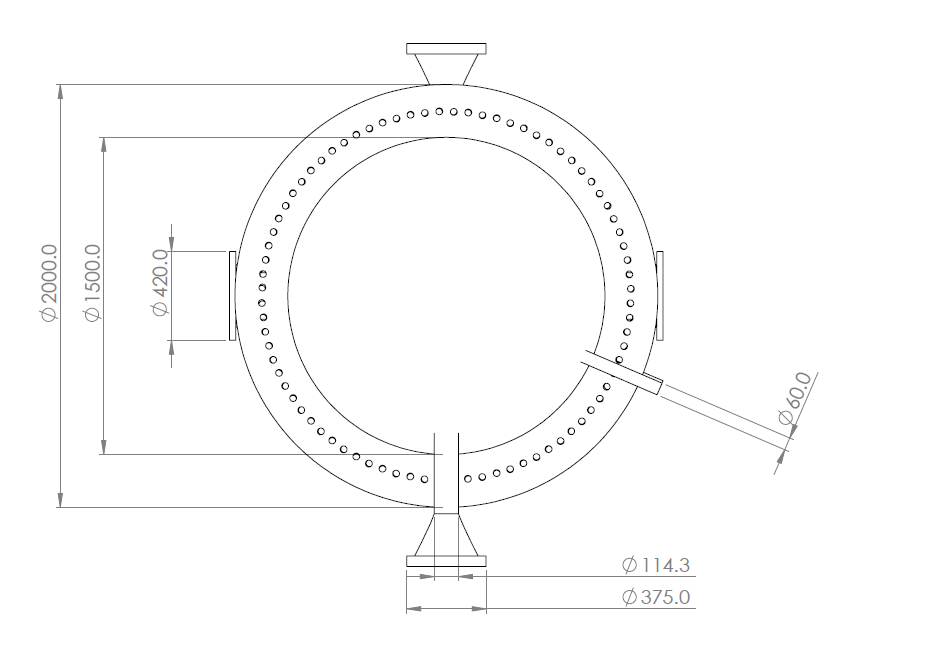
\includegraphics[width=0.6\linewidth]{chapters/2-reaction/figures/FYD reactor bottom view with calc.PNG}
    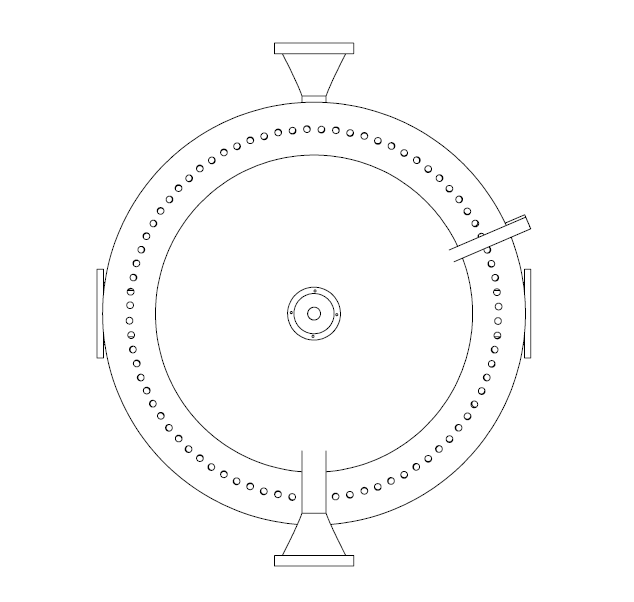
\includegraphics[width=0.49\linewidth]{chapters/2-reaction/figures/FYD reactor top view.PNG}
    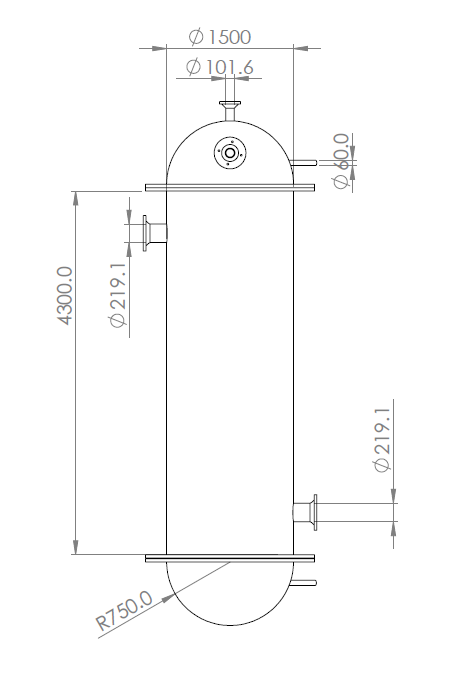
\includegraphics[width=0.49\linewidth]{chapters/2-reaction/figures/FYD reactor right view with calc.PNG}
    \caption{Top, bottom and right view of the reactor}
    \label{fig:reactortopbottomrightview}
\end{figure}

